% Rapport technique — NeuroScan (projet de module Deep Learning Avancé)
% Compilation :  python -m src.utils.report_numbers  puis  cd report && pdflatex rapport_technique.tex (x2)
\documentclass[11pt,a4paper]{article}
\usepackage[utf8]{inputenc}
\usepackage[T1]{fontenc}
% babel-french is optional: guillemets are typed directly so the file compiles without it
\IfFileExists{french.ldf}{\usepackage[french]{babel}}{}
\usepackage{lmodern}
\usepackage[margin=2.3cm]{geometry}
\usepackage{graphicx}
\usepackage{booktabs}
\usepackage{tabularx}
\usepackage{xcolor}
\usepackage{listings}
\usepackage{tikz}
\usetikzlibrary{arrows.meta,positioning,fit}
\usepackage{caption}
\usepackage{fancyhdr}
\usepackage[hidelinks]{hyperref}

\definecolor{signal}{HTML}{2E7BFF}
\definecolor{lesion}{HTML}{FF4560}
\definecolor{codebg}{HTML}{F4F6FA}
\lstset{basicstyle=\ttfamily\small,backgroundcolor=\color{codebg},frame=single,rulecolor=\color{codebg},
  columns=fullflexible,breaklines=true,keepspaces=true,showstringspaces=false,literate={é}{{\'e}}1 {è}{{\`e}}1}
\captionsetup{font=small,labelfont=bf}
\pagestyle{fancy}\fancyhf{}
\lhead{\small NeuroScan --- Détection de tumeurs cérébrales}
\rhead{\small Deep Learning Avancé}
\cfoot{\thepage}

% generated by src/utils/report_numbers.py -- do not edit
\newcommand{\fpthirtytwoPrecision}{0.450}
\newcommand{\fpthirtytwoRecall}{0.844}
\newcommand{\fpthirtytwoMapFifty}{0.492}
\newcommand{\fpthirtytwoMap}{0.353}
\newcommand{\fpthirtytwoMs}{43.3}
\newcommand{\fpthirtytwoMb}{10.7}
\newcommand{\fpsixteenPrecision}{--}
\newcommand{\fpsixteenRecall}{--}
\newcommand{\fpsixteenMapFifty}{--}
\newcommand{\fpsixteenMap}{--}
\newcommand{\fpsixteenMs}{--}
\newcommand{\fpsixteenMb}{--}
\newcommand{\inteightPrecision}{--}
\newcommand{\inteightRecall}{--}
\newcommand{\inteightMapFifty}{--}
\newcommand{\inteightMap}{--}
\newcommand{\inteightMs}{--}
\newcommand{\inteightMb}{--}
\newcommand{\pytorchPrecision}{--}
\newcommand{\pytorchRecall}{--}
\newcommand{\pytorchMapFifty}{--}
\newcommand{\pytorchMap}{--}
\newcommand{\pytorchMs}{54.9}
\newcommand{\pytorchMb}{5.5}
\newcommand{\trainPrecision}{--}
\newcommand{\trainRecall}{--}
\newcommand{\trainMapFifty}{--}
\newcommand{\trainMap}{--}
\newcommand{\trainMs}{--}
\newcommand{\trainMb}{--}
\newcommand{\modelVersion}{v2}
\newcommand{\datasetName}{Ultralytics Brain Tumor (893 train / 223 val)}

\AtBeginDocument{\renewcommand{\contentsname}{Table des matières}\renewcommand{\tablename}{Tableau}}
\newcommand{\comparisonRows}{%
yolo11n-e2-aug & yolo11n & 2 & oui & 0.452 & 0.798 & 0.479 & 0.316 & 1.5 \\
yolo11s-e50-aug & yolo11s & 50 & oui & 0.453 & 0.825 & 0.486 & 0.348 & 18.3 \\
yolo11n-e50-aug & yolo11n & 50 & oui & 0.45 & 0.833 & 0.498 & 0.359 & 11.9 \\
}

\newcommand{\code}[1]{\texttt{\detokenize{#1}}}

\begin{document}

\begin{titlepage}
  \centering
  {\large Université TEK-UP --- Cycle ingénieur IA \& Data Science, 3\textsuperscript{e} année\par}
  \vspace{2.5cm}
  {\Huge\bfseries NeuroScan\par}
  \vspace{0.4cm}
  {\Large Détection de tumeurs cérébrales sur IRM/CT\\ avec YOLO11, FastAPI, React et un cycle MLOps complet\par}
  \vspace{1.2cm}
  {\large Rapport technique --- Projet de module « Deep Learning Avancé »\par}
  {\large Axe 3 : détection d'objets en temps réel\par}
  \vfill
  \begin{tabular}{rl}
    Étudiante : & Kenza Berred \\
    Enseignant : & Haythem Ghazouani \\
    Année universitaire : & 2026--2027 \\
  \end{tabular}
  \vspace{1.5cm}

  {\small Projet pédagogique : NeuroScan n'est pas un dispositif médical.\par}
\end{titlepage}

\tableofcontents
\newpage

%-----------------------------------------------------------------------------
\section{Objectif et périmètre}
NeuroScan localise les tumeurs cérébrales sur des coupes IRM/CT et les affiche dans une application
web. Le projet couvre toute la chaîne attendue par le module :
\begin{itemize}
  \item un détecteur \textbf{YOLO11} pré-entraîné sur COCO puis fine-tuné (transfer learning) ;
  \item un pipeline \textbf{DVC} reproductible (données $\rightarrow$ entraînement $\rightarrow$ export) ;
  \item le suivi des expériences et un \textbf{Model Registry} \textbf{MLflow} ;
  \item un export \textbf{ONNX} et deux versions quantifiées (\textbf{FP16}, \textbf{INT8}) ;
  \item une API REST asynchrone \textbf{FastAPI} typée par \textbf{Pydantic} ;
  \item un client \textbf{React} (glisser-déposer, galerie d'exemples, webcam en continu) ;
  \item trois services orchestrés par \textbf{Docker Compose} et une CI/CD \textbf{GitHub Actions}.
\end{itemize}
Le choix de l'axe 3 se justifie par le besoin métier : il ne suffit pas de dire « tumeur », il
faut montrer \emph{où} elle se trouve pour qu'un radiologue puisse vérifier la zone.

\begin{figure}[h]
\centering
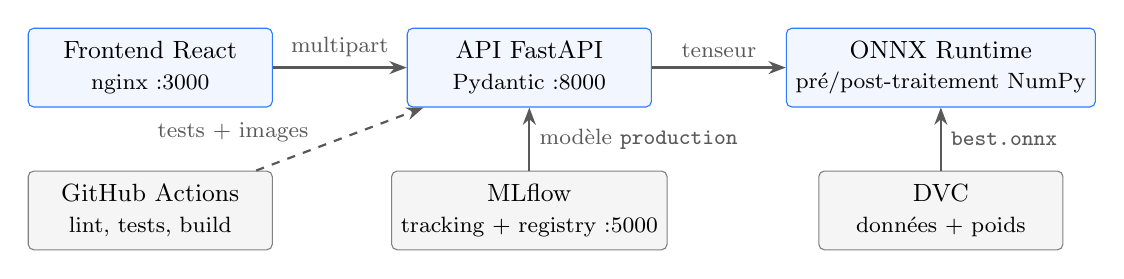
\begin{tikzpicture}[node distance=0.8cm and 1.7cm, every node/.style={font=\small},
  box/.style={draw=signal,rounded corners=2pt,minimum width=3.1cm,minimum height=1cm,align=center,fill=signal!6},
  store/.style={draw=gray,rounded corners=2pt,minimum width=3.1cm,minimum height=1cm,align=center,fill=gray!8},
  arr/.style={-{Stealth[length=2.2mm]},thick,gray!70!black}]
  \node[box] (ui) {Frontend React\\ \footnotesize nginx :3000};
  \node[box,right=of ui] (api) {API FastAPI\\ \footnotesize Pydantic :8000};
  \node[box,right=of api] (ort) {ONNX Runtime\\ \footnotesize pré/post-traitement NumPy};
  \node[store,below=of api] (mlf) {MLflow\\ \footnotesize tracking + registry :5000};
  \node[store,below=of ort] (dvc) {DVC\\ \footnotesize données + poids};
  \node[store,below=of ui] (ci) {GitHub Actions\\ \footnotesize lint, tests, build};
  \draw[arr] (ui) -- node[above]{\footnotesize multipart} (api);
  \draw[arr] (api) -- node[above]{\footnotesize tenseur} (ort);
  \draw[arr] (mlf) -- node[right]{\footnotesize modèle \code{production}} (api);
  \draw[arr] (dvc) -- node[right]{\footnotesize \code{best.onnx}} (ort);
  \draw[arr,dashed] (ci) -- node[above left=-2pt,pos=0.35]{\footnotesize tests + images} (api);
\end{tikzpicture}
\caption{Architecture découplée : trois conteneurs (frontend, API, MLflow) et le pipeline d'entraînement versionné par DVC.}
\end{figure}

%-----------------------------------------------------------------------------
\section{Données}
\subsection{Jeu de données}
Le projet utilise le jeu public \emph{Ultralytics Brain Tumor} (IRM et CT, annotations YOLO).
L'étape \code{prepare} du pipeline (\code{src/data/dataset.py}) télécharge l'archive, l'extrait dans
\code{data/brain-tumor/} et écrit le fichier \code{data.yaml}. Le jeu est fourni déjà découpé en
\emph{train} et \emph{val} : aucune normalisation ni augmentation n'est calculée sur la validation
avant le découpage, ce qui écarte la fuite de données de ce type.

\subsection{Un incident de reproductibilité, et sa correction}
Le 15 novembre 2026, Ultralytics a remplacé l'archive publiée à la même URL. La version utilisée pour
les premiers entraînements (14 novembre) comptait 2 classes (\code{negative}, \code{positive}) et
893/223 images ; la nouvelle version compte une seule classe (\code{tumor}) et 994/121 images.
Le fichier \code{dvc.lock} l'a révélé : le hash du dossier de données ne correspondait plus.

Deux corrections ont été apportées :
\begin{enumerate}
  \item l'étape \code{prepare} vérifie désormais l'empreinte MD5 de l'archive, fixée dans
        \code{params.yaml} (\code{data.md5}). Un changement en amont fait échouer le pipeline avec un
        message explicite au lieu d'entraîner en silence sur d'autres données ;
  \item un \emph{remote} DVC (\code{dvc push}/\code{dvc pull}) conserve une copie des données et des
        poids, indépendante de la source.
\end{enumerate}
Les noms de classes sont lus dans le YAML de l'archive, et l'API reconnaît \code{positive} comme
\code{tumor} : l'application fonctionne avec les deux versions du modèle.

%-----------------------------------------------------------------------------
\section{Modèle et entraînement}
\subsection{Architecture}
YOLO11 (\code{src/models/architecture.py}) est un détecteur à une étape, sans ancres : backbone CSP
(blocs C3k2), SPPF et bloc d'attention C2PSA, cou PAN, et tête de détection découplée sur trois
échelles (pas de 8, 16 et 32 pixels). Seule la branche de classification change de taille pour
nos classes ; toutes les autres couches partent des poids COCO et sont ré-entraînées de bout en bout.
Deux tailles sont comparées : YOLO11n (\(\approx\)2,6\,M paramètres) et YOLO11s (\(\approx\)9,4\,M).

\subsection{Entraînement}
Le script \code{src/models/train.py} lit \code{params.yaml} : 50 époques, images 640\(\times\)640,
batch 8, arrêt anticipé après 15 époques sans progrès, graine 42 et mode déterministe.
Les augmentations par défaut d'Ultralytics (mosaïque, mixup, variations HSV, translation, échelle,
miroir horizontal) sont actives ; \code{train.augment: false} les coupe pour l'étude d'ablation.
Chaque époque est journalisée dans MLflow (pertes, précision, rappel, mAP), ainsi que les courbes,
la matrice de confusion et les poids.

\begin{figure}[h]
\centering
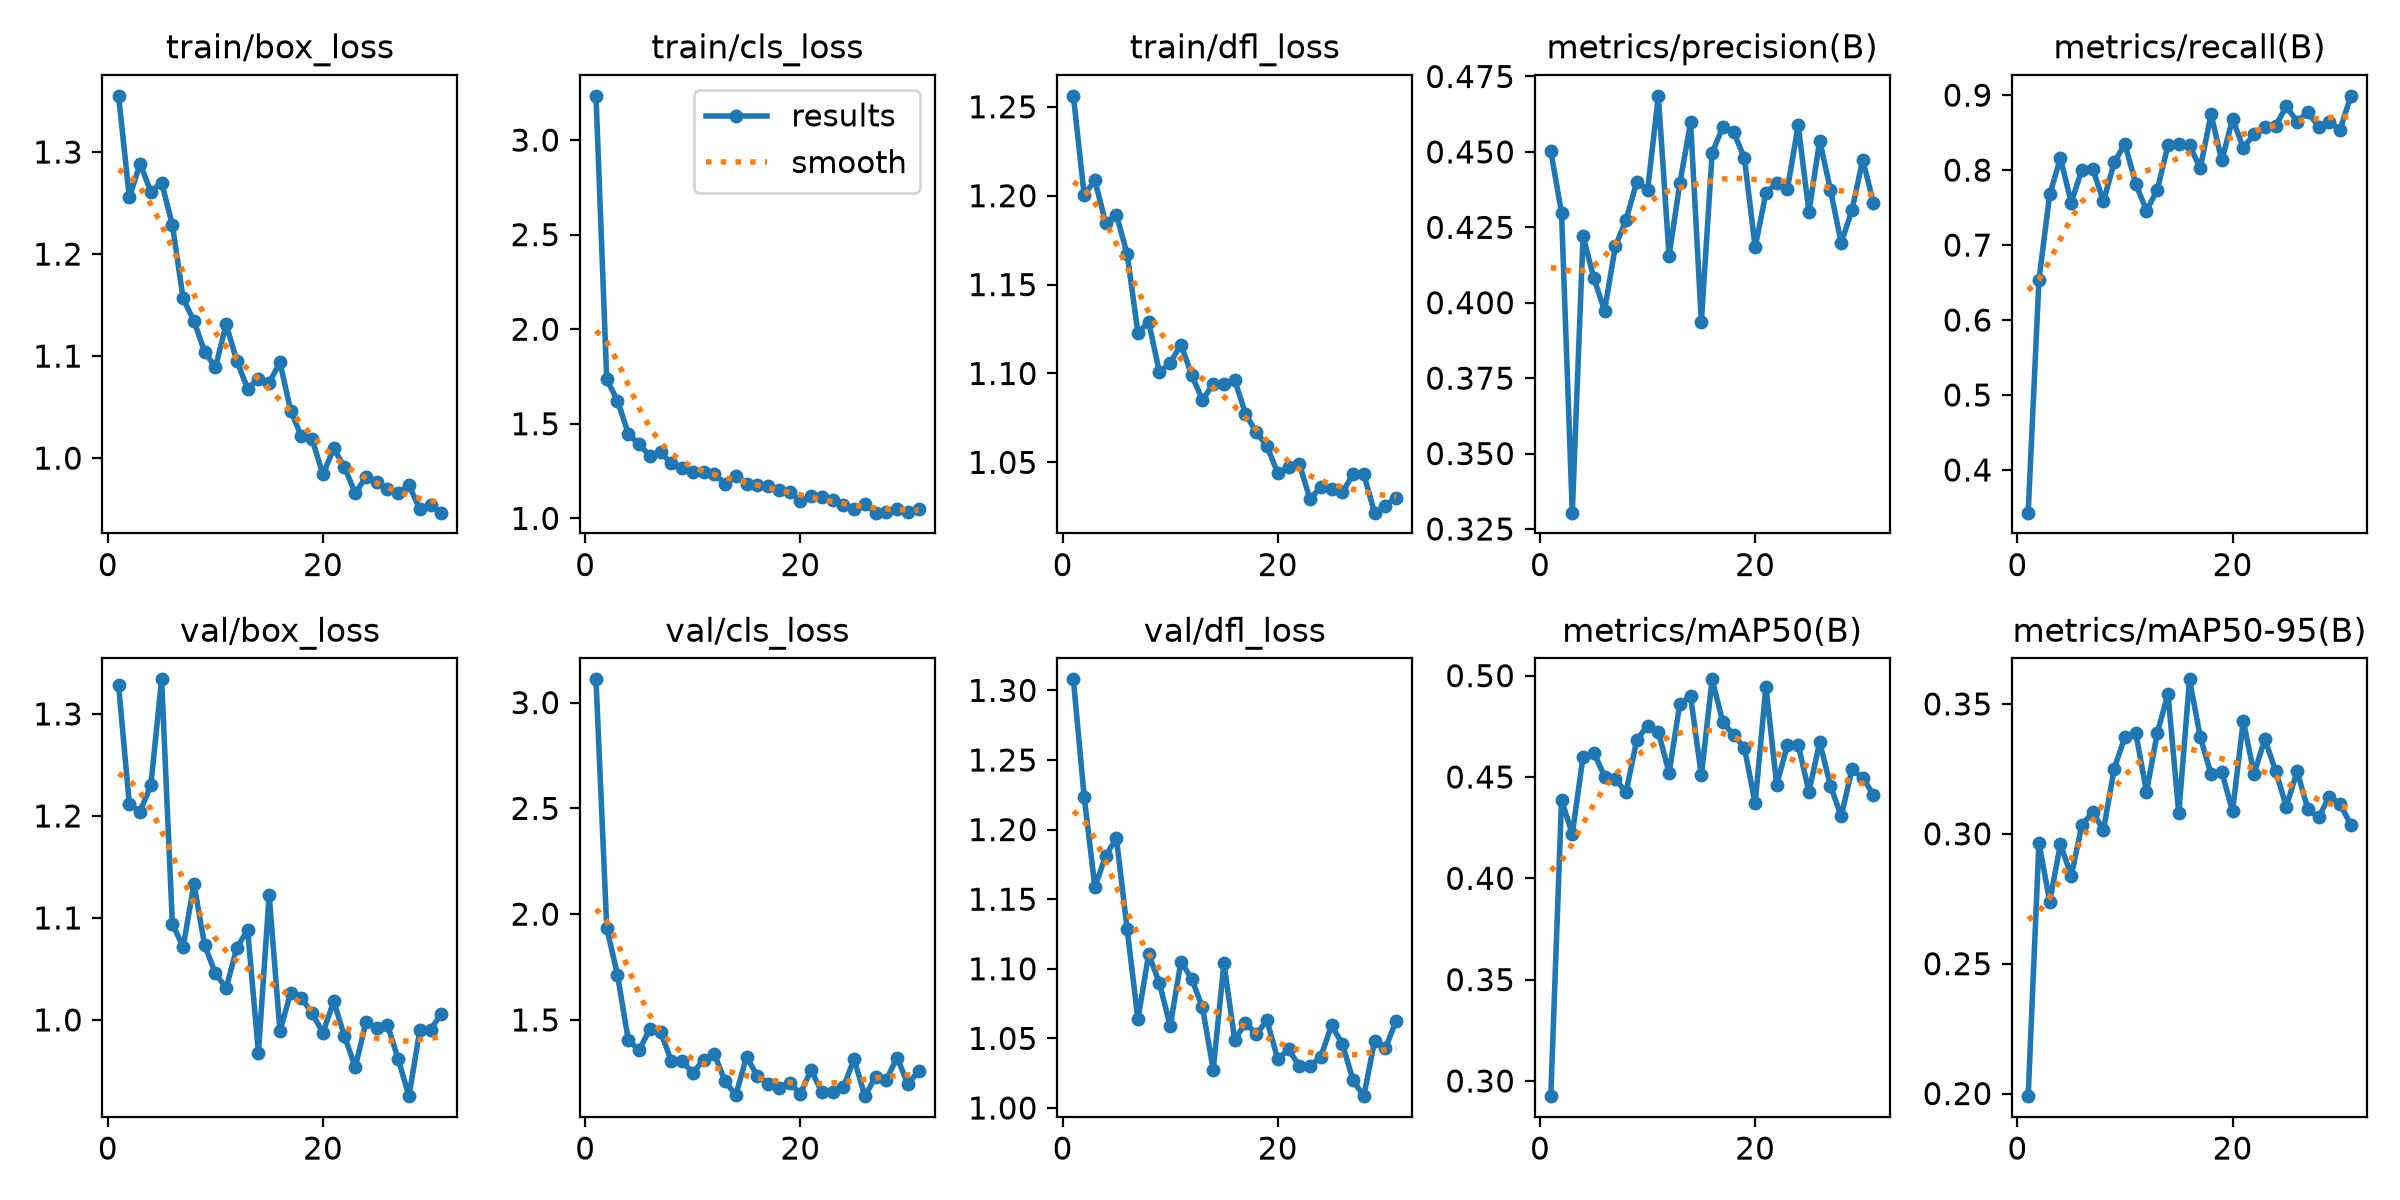
\includegraphics[width=\linewidth]{figures/results.png}
\caption{Courbes d'entraînement du modèle retenu (pertes et métriques de validation par époque).}
\end{figure}

\subsection{Analyse comparative}
Le tableau~\ref{tab:comparison} est produit par \code{python -m src.utils.compare_runs}, qui lit les
runs terminés dans MLflow. La ligne de base est un YOLO11n entraîné 2 époques ; les variantes
ajoutent l'entraînement complet, un modèle plus gros (YOLO11s) et l'ablation sans augmentation
(\code{dvc exp run --temp train -S train.augment=false}).

\begin{table}[h]
\centering\small
\begin{tabular}{lllcccccc}
\toprule
Run & Modèle & Époques & Augm. & Précision & Rappel & mAP50 & mAP50-95 & Minutes \\
\midrule
\comparisonRows
\bottomrule
\end{tabular}
\caption{Ligne de base et variantes (validation, triées par mAP50-95).}
\label{tab:comparison}
\end{table}

\begin{figure}[h]
\centering
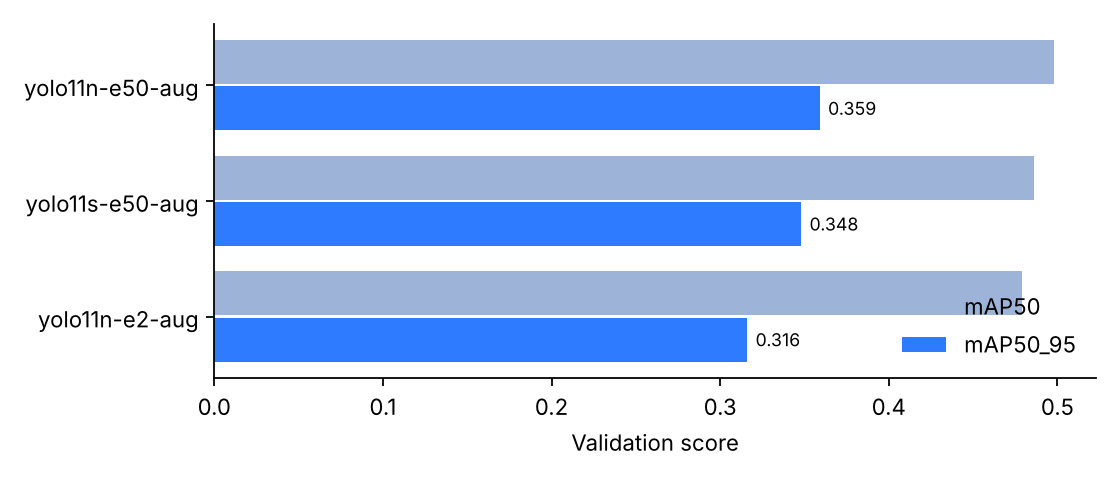
\includegraphics[width=0.72\linewidth]{figures/comparison.png}
\caption{mAP50 et mAP50-95 de chaque run.}
\end{figure}

Sur la première version du jeu de données, l'entraînement complet apporte +4,3 points de
mAP50-95 par rapport à la ligne de base. YOLO11s, 3,6 fois plus gros, ne fait pas mieux que YOLO11n :
avec moins de 900 images, la capacité supplémentaire n'est pas exploitée. YOLO11n est donc retenu,
d'autant qu'il est le plus rapide sur CPU. Le rappel (\(\approx\)0,83) est volontairement privilégié
sur la précision : manquer une tumeur coûte plus cher qu'une fausse alerte, et le seuil de confiance
reste réglable dans l'interface.

\begin{figure}[h]
\centering
\begin{minipage}{0.48\linewidth}\centering
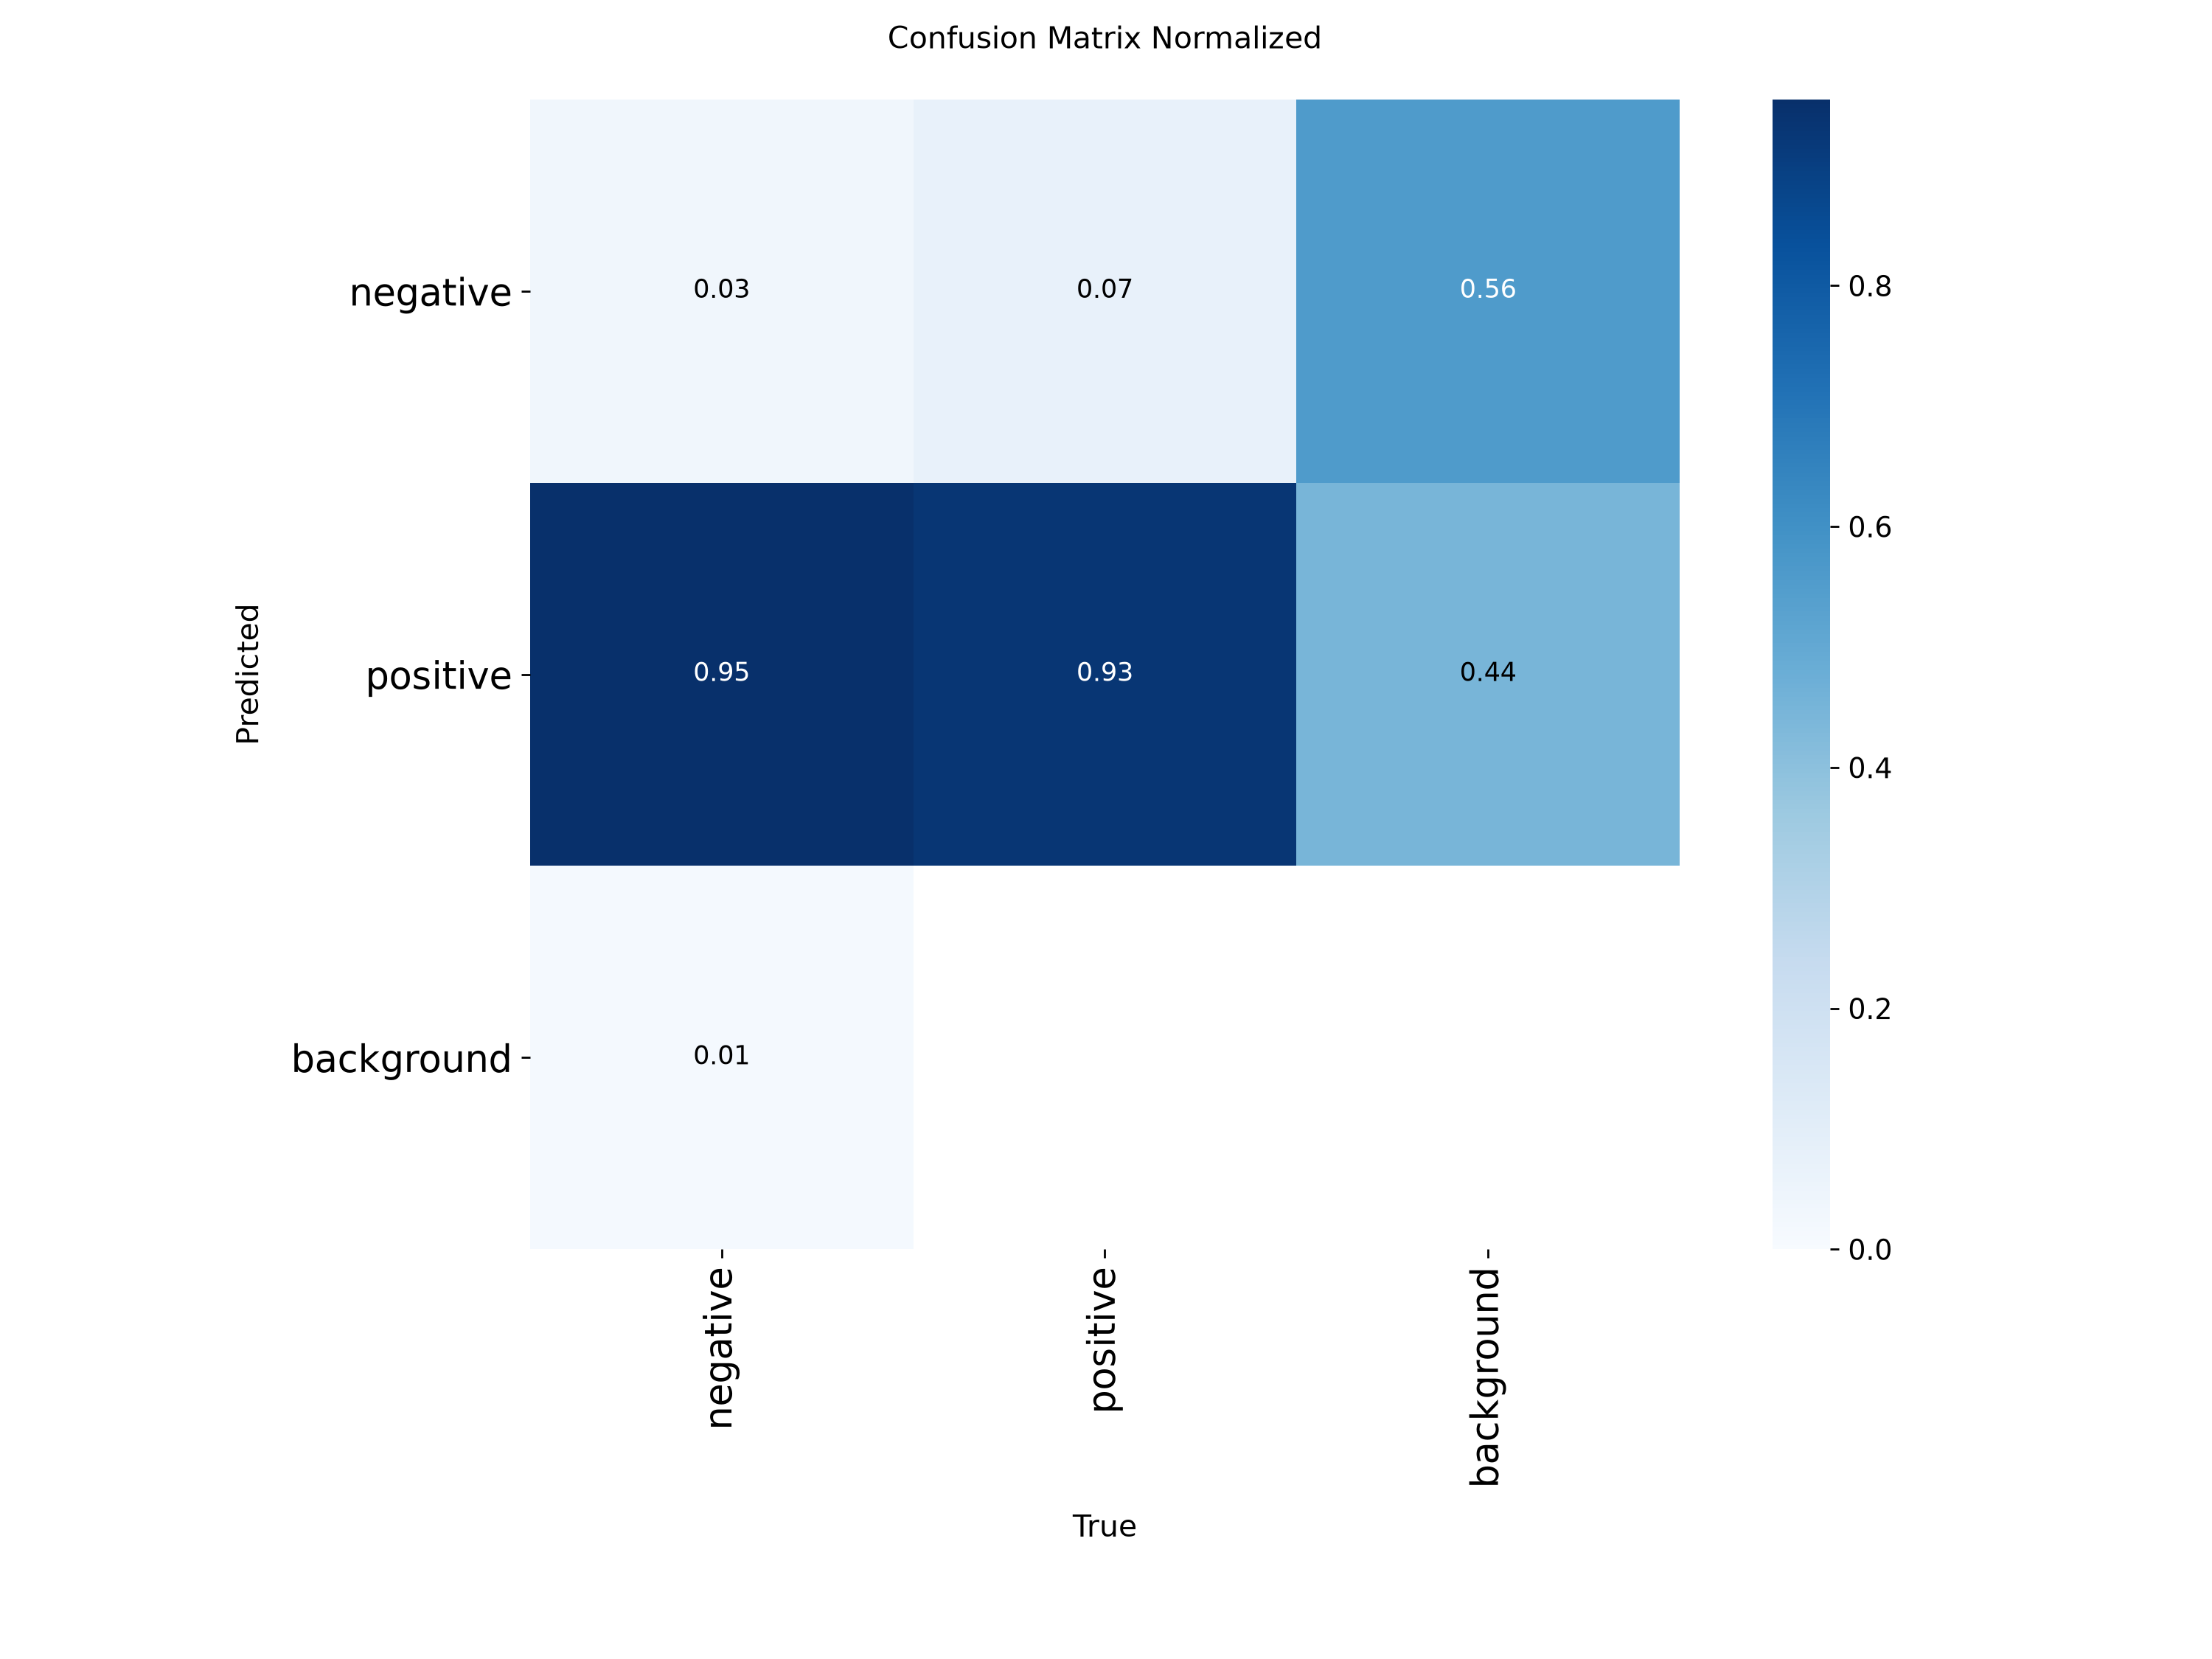
\includegraphics[width=\linewidth]{figures/confusion_matrix_normalized.png}
\end{minipage}\hfill
\begin{minipage}{0.48\linewidth}\centering
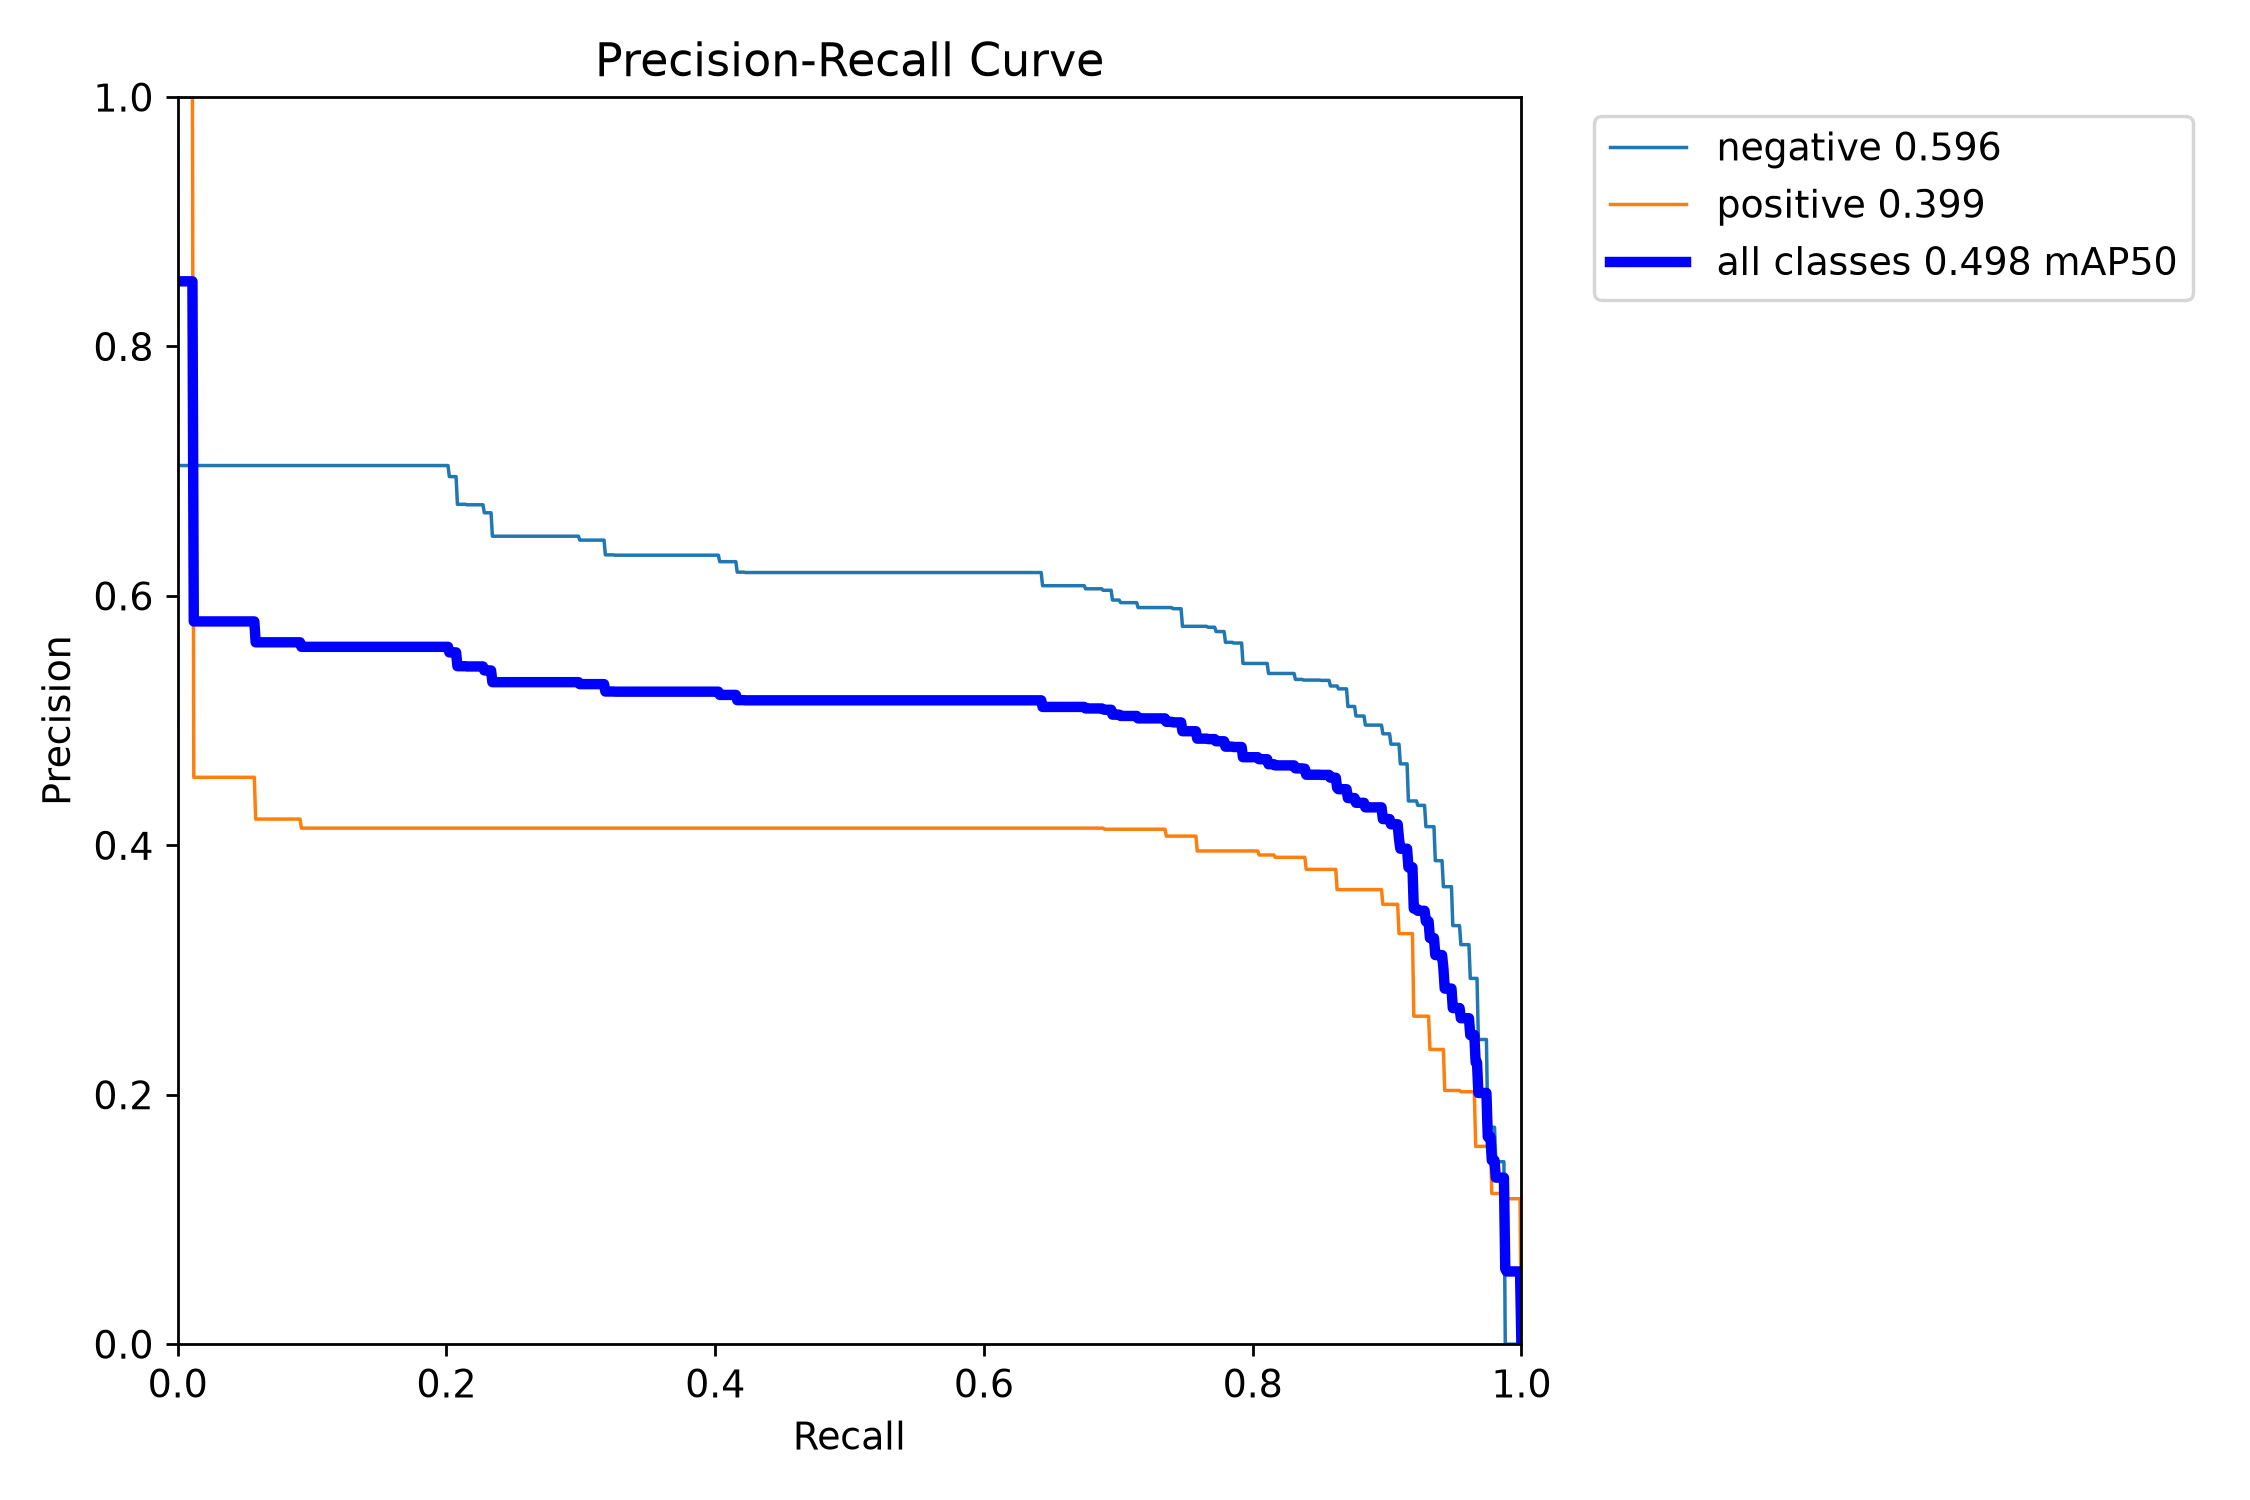
\includegraphics[width=\linewidth]{figures/BoxPR_curve.png}
\end{minipage}
\caption{Matrice de confusion normalisée et courbe précision-rappel du modèle retenu.}
\end{figure}

%-----------------------------------------------------------------------------
\section{Optimisation pour l'inférence}
L'étape \code{export} (\code{src/models/evaluate.py}) exporte le meilleur checkpoint en ONNX
(opset 12, graphe simplifié), puis produit deux variantes :
\begin{itemize}
  \item \textbf{FP16} : poids et activations en demi-précision ; entrées et sorties restent en FP32
        pour l'API ;
  \item \textbf{INT8} : quantification statique (format QDQ, poids par canal), calibrée sur 100 images
        d'entraînement. Le décodage final de la tête (DFL, ancres, concaténation des boîtes en pixels et
        des scores entre 0 et 1) reste en FP32 : une seule échelle INT8 ne peut pas couvrir ces deux
        plages, et sans cette exclusion le rappel s'effondrait (0,13 au lieu de 0,76 lors d'un essai).
\end{itemize}
Les trois modèles sont évalués sur la validation \emph{avec le code d'inférence de l'API}
(fichier \code{inference.py} du backend) et des métriques écrites en NumPy (\code{metrics.py}).
Ces métriques ont été vérifiées contre \code{ap_per_class} d'Ultralytics sur les mêmes prédictions (écart
inférieur à 0,001 de mAP50).

\begin{table}[h]
\centering\small
\begin{tabular}{lccccc}
\toprule
Modèle & mAP50 & mAP50-95 & Rappel & Latence CPU (ms) & Taille (Mo) \\
\midrule
PyTorch (\code{best.pt}) & --- & --- & --- & \pytorchMs & \pytorchMb \\
ONNX FP32 (servi) & \fpthirtytwoMapFifty & \fpthirtytwoMap & \fpthirtytwoRecall & \fpthirtytwoMs & \fpthirtytwoMb \\
ONNX FP16 & \fpsixteenMapFifty & \fpsixteenMap & \fpsixteenRecall & \fpsixteenMs & \fpsixteenMb \\
ONNX INT8 & \inteightMapFifty & \inteightMap & \inteightRecall & \inteightMs & \inteightMb \\
\bottomrule
\end{tabular}
\caption{Précision et vitesse des variantes (médiane sur 30 images de validation, pré-traitement,
modèle et NMS compris). Valeurs écrites par \code{dvc repro} dans \code{reports/export.json}.}
\end{table}

Lors des essais, l'INT8 était 1,6 fois plus rapide et 3,3 fois plus léger que le FP32, pour moins
d'un point de mAP50 perdu. Le FP16 divise la taille par deux mais n'accélère pas sur CPU (le
matériel ne calcule pas nativement en demi-précision) ; il est destiné à un GPU. Le FP32 reste servi
par défaut ; l'INT8 peut être servi en changeant \code{MODEL_PATH}.

%-----------------------------------------------------------------------------
\section{Cycle MLOps}
\subsection{DVC}
\code{dvc.yaml} décrit trois étapes et leurs dépendances (code, données, paramètres) :
\begin{lstlisting}
prepare  : python -m src.data.dataset    -> data/brain-tumor
train    : python -m src.models.train    -> models/best.pt, reports/metrics.json
export   : python -m src.models.evaluate -> models/best*.onnx, reports/export.json
\end{lstlisting}
\code{dvc repro} ne relance que les étapes dont une dépendance a changé ; \code{dvc.lock} enregistre
les hash de chaque entrée et sortie. Les données et les poids ne sont jamais dans Git ; ils sont
poussés sur le remote DVC (\code{dvc push}).

\subsection{MLflow}
Chaque entraînement crée un run : hyperparamètres, nombre de paramètres du réseau, métriques par
époque et finales, figures, poids. L'export ajoute au même run les métriques des trois variantes et
enregistre le modèle ONNX FP32 dans le registry \code{brain-tumor-detector}. La nouvelle version reçoit
l'alias \code{production} et le stage « Production » ; les précédentes passent en « Archived ».

\begin{figure}[h]
\centering
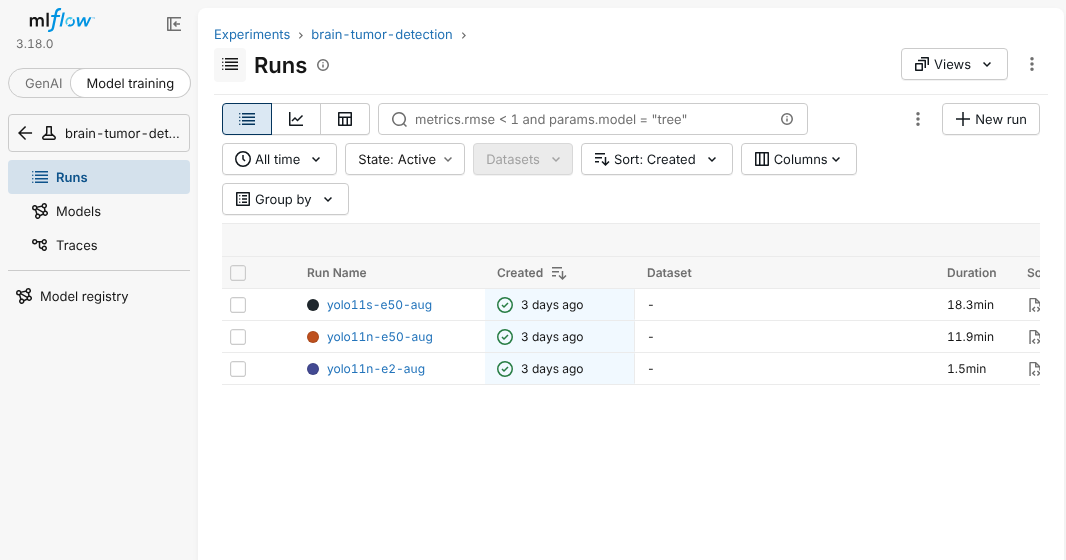
\includegraphics[width=\linewidth]{figures/mlflow_runs.png}
\caption{Runs de l'expérience \code{brain-tumor-detection} dans MLflow.}
\end{figure}

\begin{figure}[h]
\centering
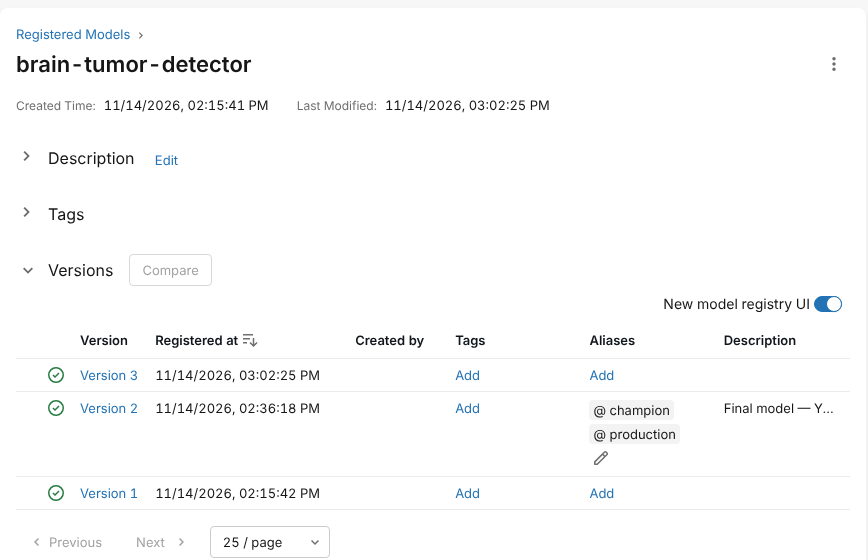
\includegraphics[width=0.8\linewidth]{figures/mlflow_registry.png}
\caption{Model Registry : la version servie porte l'alias \code{production}.}
\end{figure}

\subsection{Conteneurs et CI/CD}
\code{docker compose up --build} démarre MLflow (5000), l'API (8000) et le frontend (3000). Les deux
Dockerfiles sont multi-étapes : l'API installe ses dépendances dans un environnement virtuel jeté
ensuite et s'exécute sous un utilisateur non-root ; le frontend est compilé par Node puis servi par
nginx. L'image de l'API n'embarque ni PyTorch ni Ultralytics.

Deux workflows GitHub Actions s'exécutent à chaque push :
\begin{itemize}
  \item \code{ci-tests.yml} : ruff (lint et format) et 22 tests pytest pour l'API, ESLint et build pour
        le frontend, ruff pour le code d'entraînement, et validation du graphe DVC (\code{dvc dag}) ;
  \item \code{docker-build.yml} : build des images et test de fumée de l'API conteneurisée
        (\code{/health}).
\end{itemize}

%-----------------------------------------------------------------------------
\section{Application}
\subsection{API FastAPI}
\begin{table}[h]
\centering\small
\begin{tabularx}{\linewidth}{llX}
\toprule
Méthode & Route & Rôle \\
\midrule
GET & \code{/health} & état du serveur, GPU disponible, version du modèle chargé \\
GET & \code{/model/metadata} & nom, architecture, classes, métriques de validation, benchmark \\
POST & \code{/predict} & image $\rightarrow$ boîtes, classes et scores en JSON + temps d'inférence \\
POST & \code{/predict/visualize} & image $\rightarrow$ PNG annoté (une couleur par classe) \\
\bottomrule
\end{tabularx}
\caption{Routes de l'API (documentation Swagger sur \code{localhost:8000/docs}).}
\end{table}

Toutes les réponses sont validées par des schémas Pydantic. Le modèle est chargé une seule fois au
démarrage et l'inférence s'exécute dans un thread pour ne pas bloquer la boucle asynchrone. Les erreurs
utilisent des codes HTTP explicites : 400 (image illisible), 413 (fichier trop lourd), 415 (pas une
image), 422 (paramètre invalide), 503 (modèle non chargé). Le pré-traitement (letterbox), le décodage de
la tête YOLO11 et la NMS sont réécrits en NumPy ; sur les mêmes images, ils donnent exactement les mêmes
prédictions qu'Ultralytics.

\begin{figure}[h]
\centering
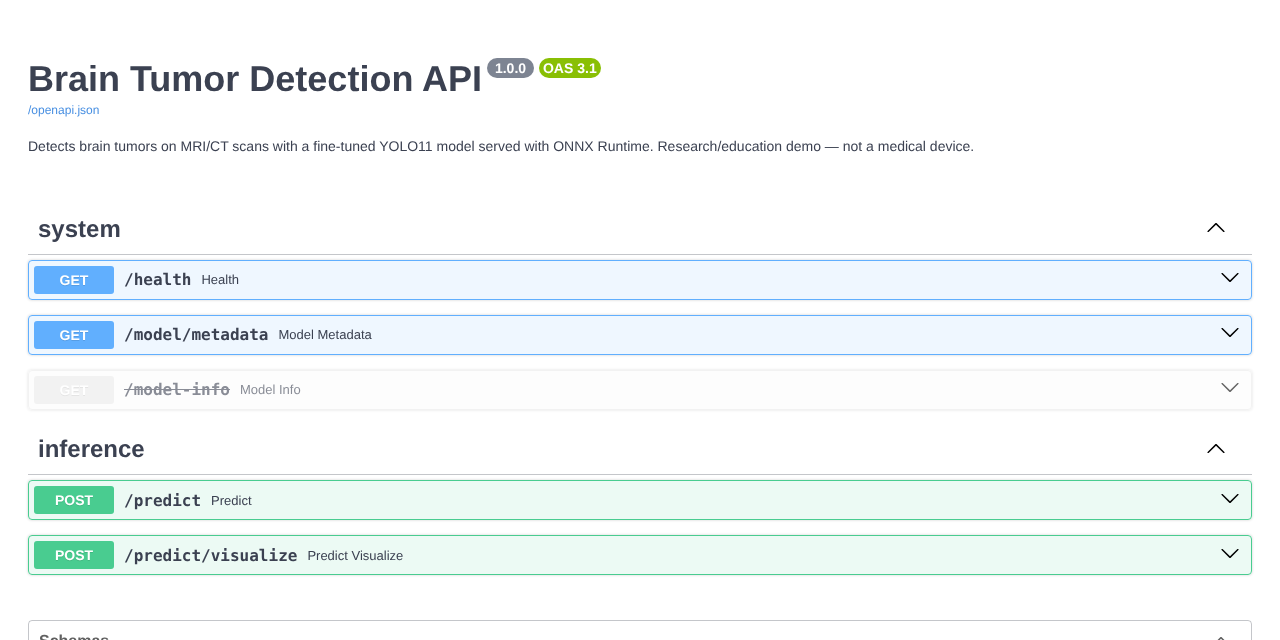
\includegraphics[width=0.85\linewidth]{figures/swagger.png}
\caption{Documentation Swagger générée par FastAPI.}
\end{figure}

\subsection{Frontend React}
L'interface (Vite, React 18, Tailwind CSS v4 pour le panneau de résultats) propose trois modes
d'entrée : glisser-déposer, galerie de huit images d'exemple et webcam en flux continu. Les boîtes
sont dessinées sur un canvas superposé, avec label et score. Les scores s'affichent en barres de
progression animées, et deux latences sont mesurées : le temps du modèle côté serveur et l'aller-retour
complet mesuré dans le navigateur. Les chiffres de la page d'accueil sont lus en direct sur
\code{/model/metadata}.

\begin{figure}[h]
\centering
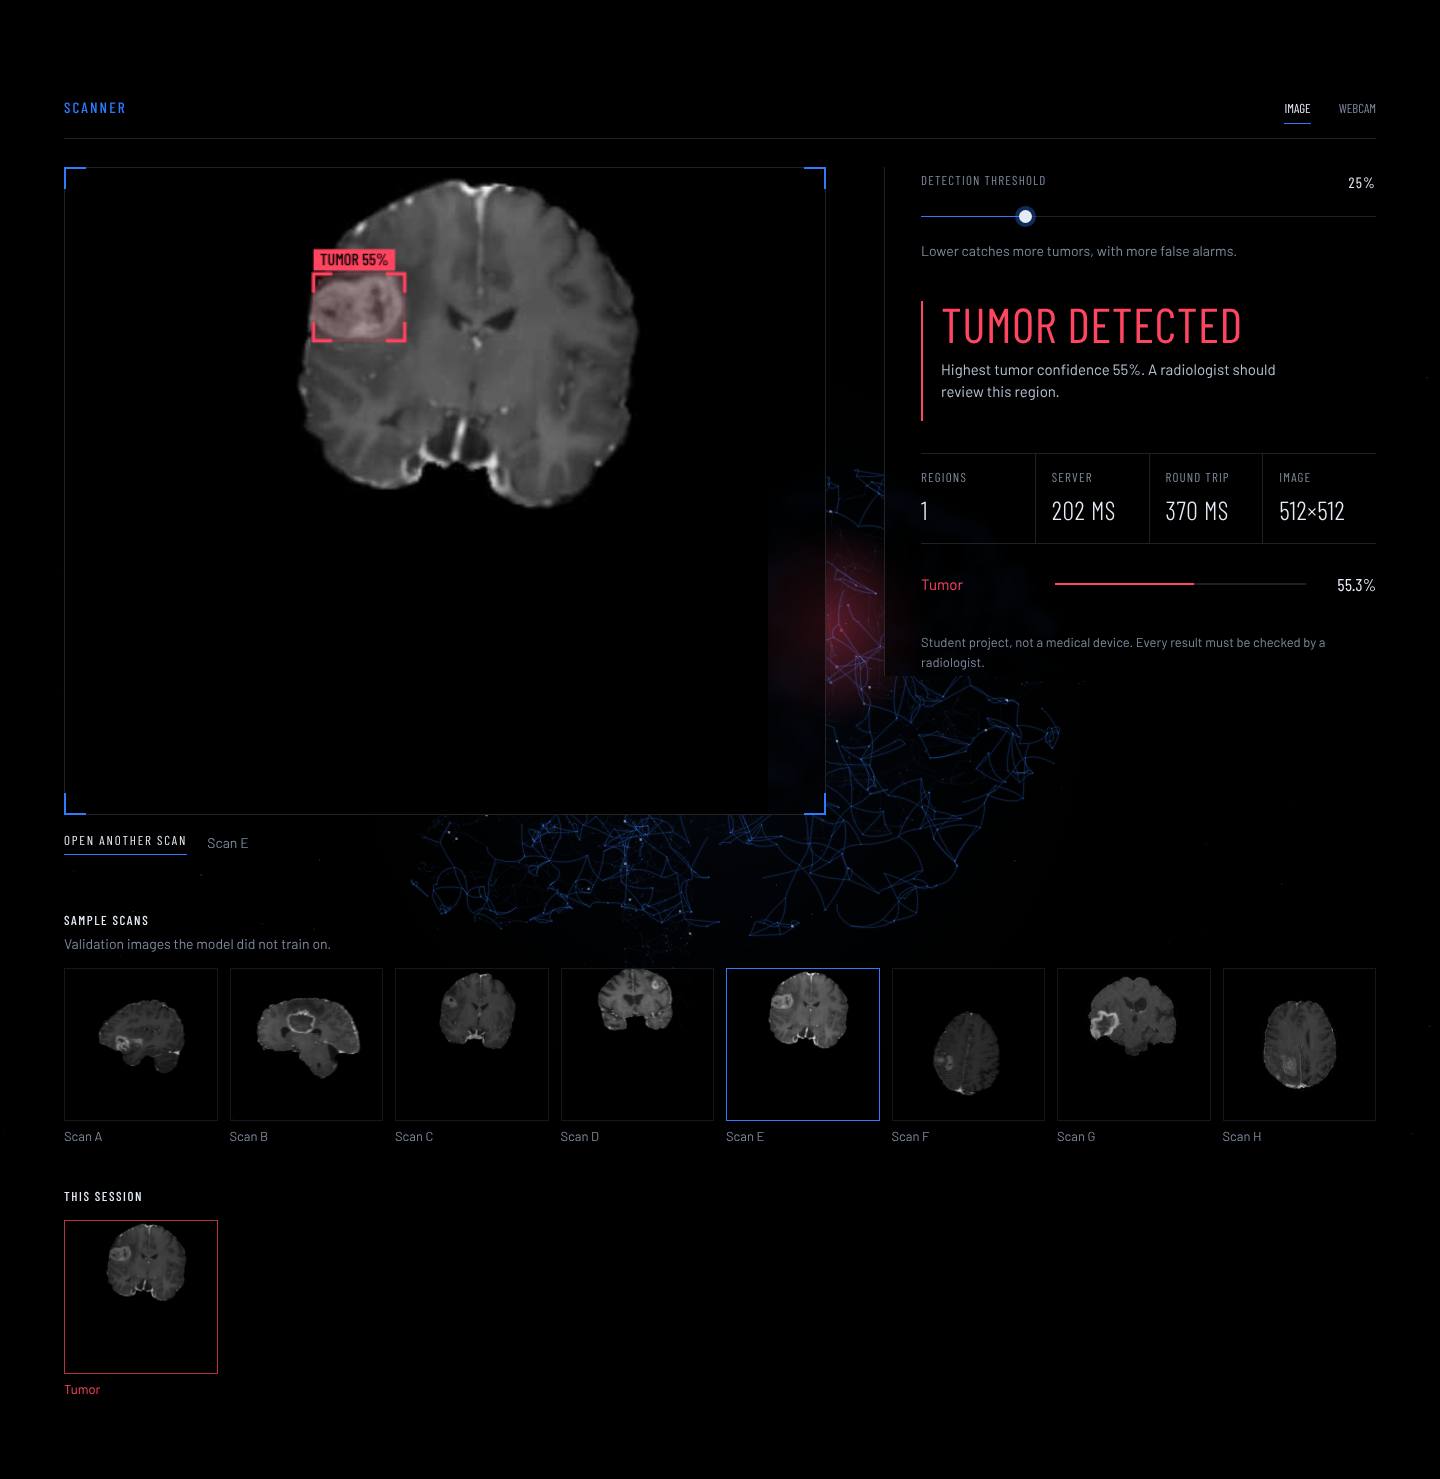
\includegraphics[width=0.9\linewidth]{figures/scanner.png}
\caption{Analyse d'une image d'exemple : boîte, verdict, latences serveur et aller-retour, score.}
\end{figure}

%-----------------------------------------------------------------------------
\section{Limites et perspectives}
\begin{itemize}
  \item Le découpage train/val n'est pas fait par patient : des coupes d'un même patient peuvent se
        trouver des deux côtés, ce qui rend les scores possiblement optimistes.
  \item Le jeu de données est petit (environ 1\,100 images) ; une validation croisée ou un jeu de test
        externe donnerait une estimation plus fiable.
  \item Le monitoring en production (dérive des données, Prometheus/Grafana) n'est pas encore en place.
  \item L'INT8 pourrait devenir le modèle servi après une validation sur plus d'images.
\end{itemize}

\end{document}
